\documentclass[12pt]{report}
\usepackage{url}
\usepackage{xcolor}
\usepackage{apacite}
\usepackage{caption}
\usepackage{amsmath}
\usepackage{pgfgantt}
\usepackage{mathptmx} 
\usepackage{graphicx}
\usepackage{indentfirst}
\usepackage{subcaption}
\usepackage[utf8]{inputenc}
\usepackage[english]{babel}
\usepackage{ragged2e}
\usepackage[nottoc,notlof,notlot]{tocbibind} 
\usepackage[a4paper, total={6in, 8in}]{geometry}
\usepackage[explicit]{titlesec}
\titleformat{\chapter}
[display]{\bfseries\centering}
{\huge Chapter \thechapter}
{1em}{\Huge #1}


\definecolor{tail}{RGB}{26, 188, 156}
\geometry{margin=1in}
\linespread{2}

\justifying
\setlength{\parindent}{2em}

%\setlength{\parskip}{1em}
% \title{Sign language recognition using deep learning}
% \author{ Name: MHD Khaled Maen\\
%     Matric No: 1523592 \\ 
%     [1.5cm]
%     Supervised by\\
%     Assoc. Prof. Dr. Amelia Ritahani \\} 
% \date{\today} 
\begin{document}
\begin{titlepage}
    \center
    
\includegraphics[width = 15 cm]{./images/iium.png}
    \textsc{\LARGE }\\[1 cm]
    \textsc{\LARGE kulliyyah of information and}\\[.1 cm]
    \textsc{\LARGE communication technology}\\[1 cm]
    \textsc{\Large department of computer science}\\ [ .2 cm]
    \textsc{\large fyp preliminary report}\\ [.5 cm]
    \hrulefill \\[0.2cm]
    \textsc{\Large sign language recognition using deep learning}\\
    \hrulefill \\[1 cm]
    
    \textsc{\large mhd khaled maen}\\[.1 cm]
    \textsc{1523591}\\ [1 cm]
    
    
    \textsc{\large supervised by}\\[.1 cm]
    \textsc{\large assoc. prof. dr. amelia ritahani}\\[2 cm]
    
    \textsc{\large december} 2018\\ [.2 cm]
    \textsc{\large semester} 1, 2018 / 2019 \\
    
\end{titlepage}

\pagenumbering{roman}
% \maketitle
\begin{center}
    \LARGE DECLARATION
\end{center}   

I hear by declare that this report is the result of my own investigations,
except where otherwise stated. I also clear that it 
has not been previously or currently submitted as a whole for any other degree 
at IIUM or other institutions.

\mbox{}
\vfill
MHD KHALED MAEN (1523591)
\bigbreak
Signature: .................\hspace{18em} Date: .................
\bigbreak

\newpage
\begin{center}
    \LARGE APPROVAL PAGE
\end{center} 

I certified that I have supervise can read this study and that in my opinion,
confirms to acceptable standards of scholarly presentation and is fully adequate,
in scope and quality, as final year project paper a partial fulfilment for a 
degree of bachelor of Computer Science (Honours).
\mbox{}
\vfill
Assoc. Prof. Dr. Amelia Ritahani (Supervisor)
\bigbreak
Department of Computer Science
\bigbreak
Kulliyyah of Information and Communication Technology
\bigbreak
International Islamic University Malaysia
\bigbreak

\newpage

\begin{center}
    \LARGE ABSTRACT
\end{center}

Communication is an essential part of our life.
Unfortunately, some of us were born in various types of disability such as deaf,
since hearing impaired people can't listen they can't learn to speak so they developed 
a new communication why to interact with other people by using distinct hand gestures, 
which wasn't enough to overcome this issue, even now with all technologies and tool still challenging problem to solve.
For the mentioned reason, 
the intention of the proposed research is to improve an ordinary model to translate the hand gestures of the sign language into voice.
In that, Deep learning is remarkably serviceable for this mission, 
firstly by identifying the hand in the video frame by using Convolutional
Neural Network algorithm then states the sound that matches the sign.The accuracy achieved for detect hand gesture using initial CNN model 92 \text{\%} for MNIST
dataset and 82\text{\%} for regular dataset.


\newpage
\begin{center}
    \LARGE ACKNOWLEDGEMENT
\end{center} 

This project has been completed with support from my supervisor, Assoc. Prof. Dr. Amelia Ritahani, many thanks for her wonderful 
collaboration and consultation sessions. Furthermore, 
I would like to thank my coordinator, Asst. Prof. Dr. Hamwira Yaacob, for his 
assistance helping me and others by organizing weekly sessions towards writing perfect report step-by-step. 
Last but not least,
I want to thank my awesome parents for their support and time helping me reach the end of my undergraduate study, without them, I could not achieve that.

\setcounter{page}{2}                    
\tableofcontents{}
\listoffigures
\listoftables
\newpage

\pagenumbering{arabic}
\chapter{Introduction} 

\section{Background}
Communication is a process of sending and receiving data among individuals. 
People communicate with o with a considerable measure of ways yet the best way is eye to eye correspondence.
Numerous individuals trust that the significance of communication 
is like the importance of breathing. Indeed, communication facilitates the spread of knowledge
and structures connections between individuals.

Deep learning added an immense lift to the already rapidly developing field of computer vision.
With deep learning, a lot of new utilization of computer vision techniques have been presented
and they are currently ending up some portion of our regular day to day existence.

Alongside with the intensity of the present computers, there are now various algorithms that were developed 
to empower the computers to perform tasks such as object tracking and pattern recognition. 

In this study, the attention will be on hand gestures detection and make an interpretation of them into voice.

\section{Problem Statement}
Communication difficulties arising from damage to hearing
directly have an effect on the standard of life. Difficulties in communication could
end in deviations within the emotional and social development which
will have a major impact on the standard of lifetime of every one.
It is well recognized that hearing is crucial to speech and language development, communication, and learning.
Folks with listening difficulties due to hearing loss or auditory processing problems
continue to be an under-identified and under-served population. The
earlier the matter is known and intervention began, the less
serious the ultimate impact \cite{AFrajtag12017}.

The communication between hearing-impaired and other individuals is a colossal gab 
need to be filled up. In order to overcome this challenge 
many researches and products have been developed to solve this problem, 
but there is a lot to be enhanced.

\section{Objectives}
\begin{itemize}
    \item To study sign language gestures.
    \item To develop a new hand gesture into voice algorithm.
    \item To construct a hand gesture into voice model.
\end{itemize}

\section{Scope}
This research aims to develop a sign language recognition algorithm,
and converting it into voice.
\section{Significance}
Help the hearing-impaired community to communicate with hearing ones, 
in order to make a strong connected community.

\section{Timeline}
\begin{center}
    \begin{ganttchart}[
        expand chart=\textwidth,
        bar/.append style={draw=none, fill=tail},
        hgrid style/.style={draw=black!5, line width=.75pt},
        vgrid={*1{draw=black!5, line width=.75pt}},
        ]{1}{14}
        \gantttitle{Week}{14} \\
        \gantttitlelist{1,...,14}{1} \\
        \ganttbar{Title Selectin}{1}{3}  \\
        \ganttbar{Overall System Review}{2}{7}  \\
        \ganttbar{Literature Review}{4}{12}  \\
        \ganttbar{System Design}{8}{11}  \\
        \ganttbar{Design \& Prototype}{9}{12}  \\
        \ganttbar{Simulation}{7}{13}  \\
        \ganttbar{Report Writing}{5}{13}  \\
        \ganttbar{Submission}{13}{13}  \\
    \end{ganttchart}
\end{center}
\chapter{Literature review}

This chapter includes reviews of other previous researcher
and their proposed methods they used in implementing deep learning
to recognize hand gestures. These researches will help to grasp the knowledge
to achieve the project's objectives. 

\section{Previous works}

\cite{Bao2017}, proposed a Deep convolutional neural network algorithm for hand-gesture 
recognition without hand localisation, since the hands only occupy about 10\% of 
the image. They used a combination of 9 convolution layers, 3 fully connected layers, 
interlaced with ReLU(Rectified Linear Unit) and dropout layers as shown in 
figure \ref{fig:tiny_architecture}. Alongside this architecture the apply some image 
processing techniques to have sufficient computation efficiency and memory requirement.
According to the paper the accuracy achieved was 97.1\% in the images with simple backgrounds
and 85.3\% in the images with complex backgrounds.However, the main disadvantage of of 
the proposed algorithm is the training set which only includes 7 different gestures,
and it tends to have bad accuracy with complex backgrounds.
\bigbreak

\begin{figure}[h]
    \centering
    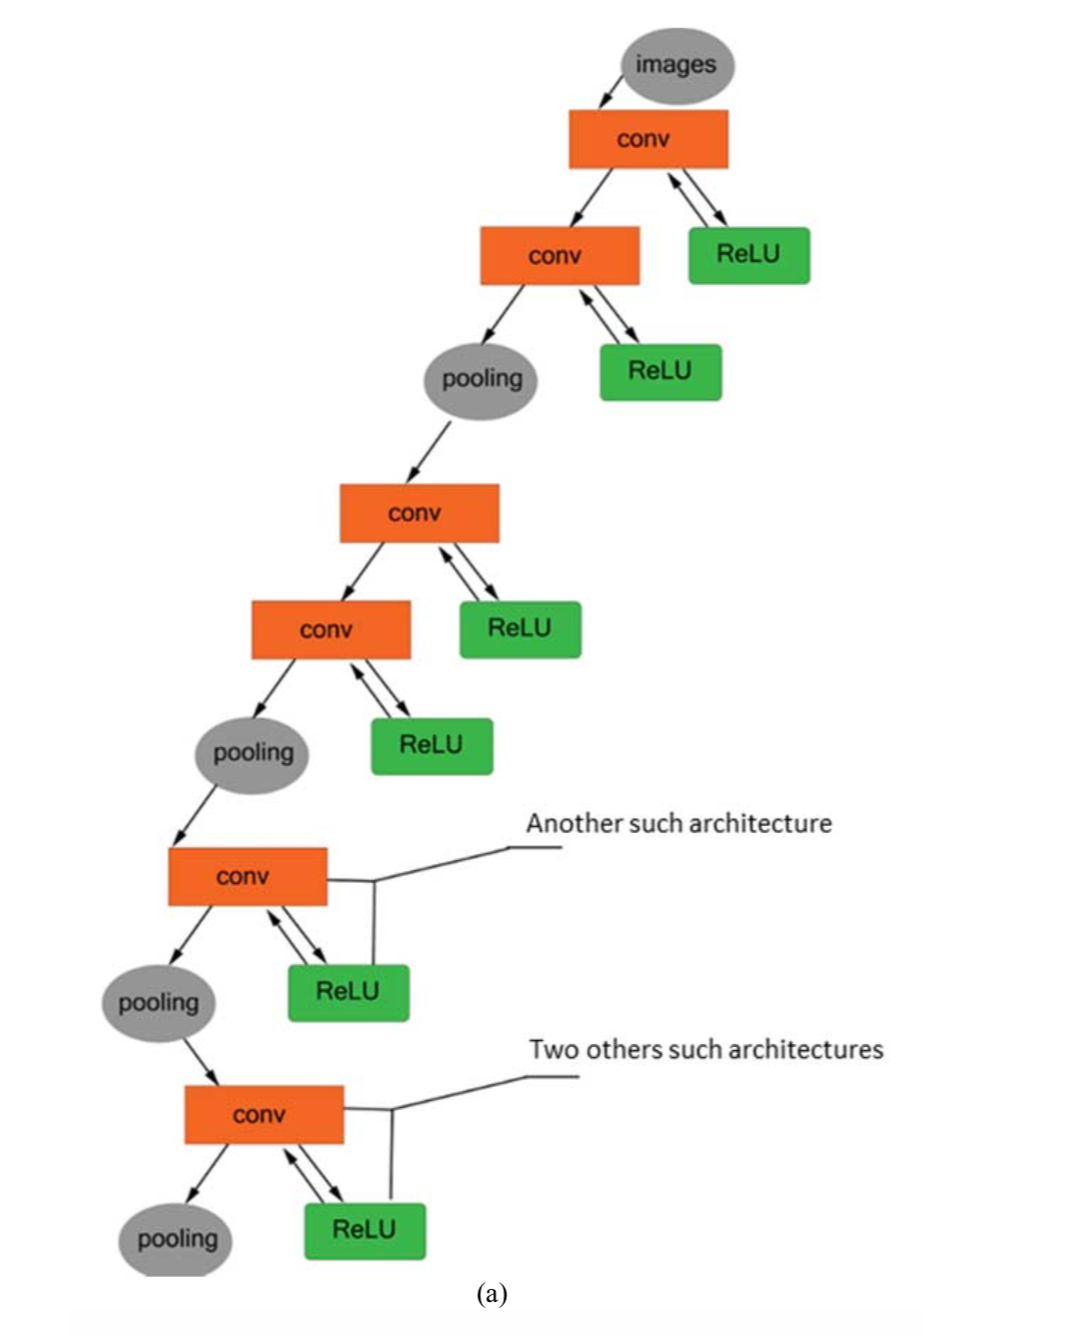
\includegraphics[width=.8\textwidth]{./images/tiny_a.png}
\end{figure}
\bigbreak
\begin{figure}
    \centering
    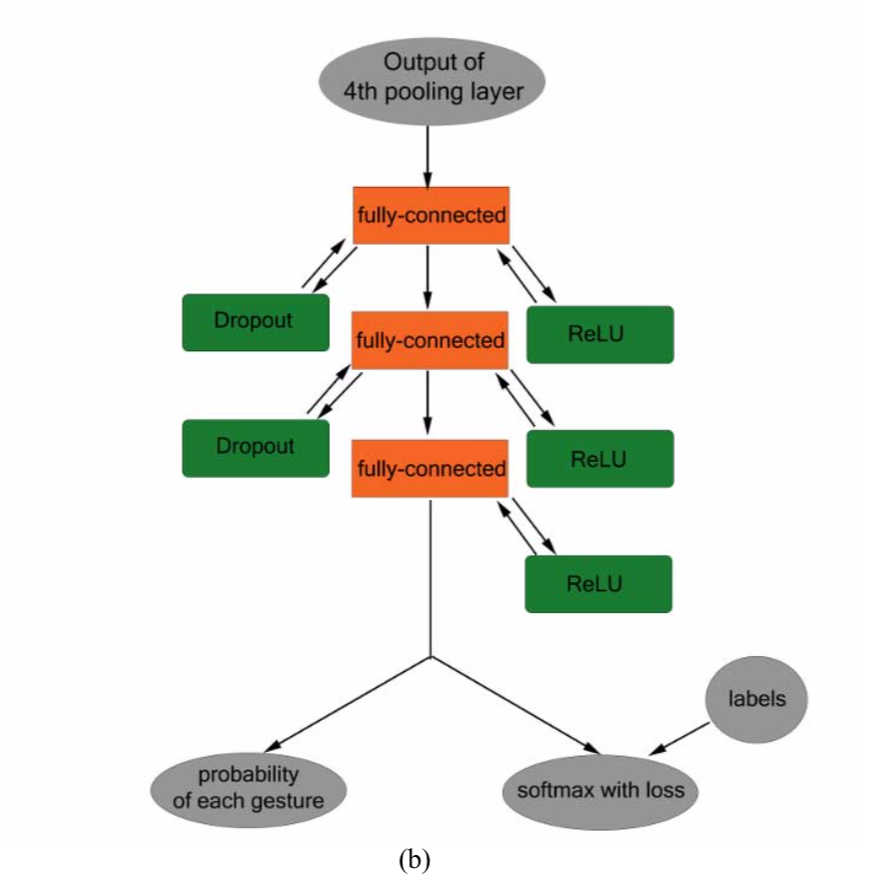
\includegraphics[width=\textwidth]{./images/tiny_b.png}
    \caption{Architecture of the proposed deep CNN }\label{fig:tiny_architecture}
\end{figure}

\clearpage

\cite{Rao2018}, proposed a CNN architecture for classifying selfie sign language gestures. 
The CNN architecture is designed with four convolutional layers. Each convolutional 
layer with different filtering window sizes as shown in figure \ref{fig:selfie}  
They had a dataset with five different subjects performing 200 signs in 5 different viewing angles 
under various background environments. Each sign occupied for 60 frames or images in a video.
The proposed model performed training on 3 batches to test the robustness of different training mode 
using caffe deep learning framework. However, the result accuracy was 92.88\% need more training and improvements. 

\begin{figure}[h]
    \centering
    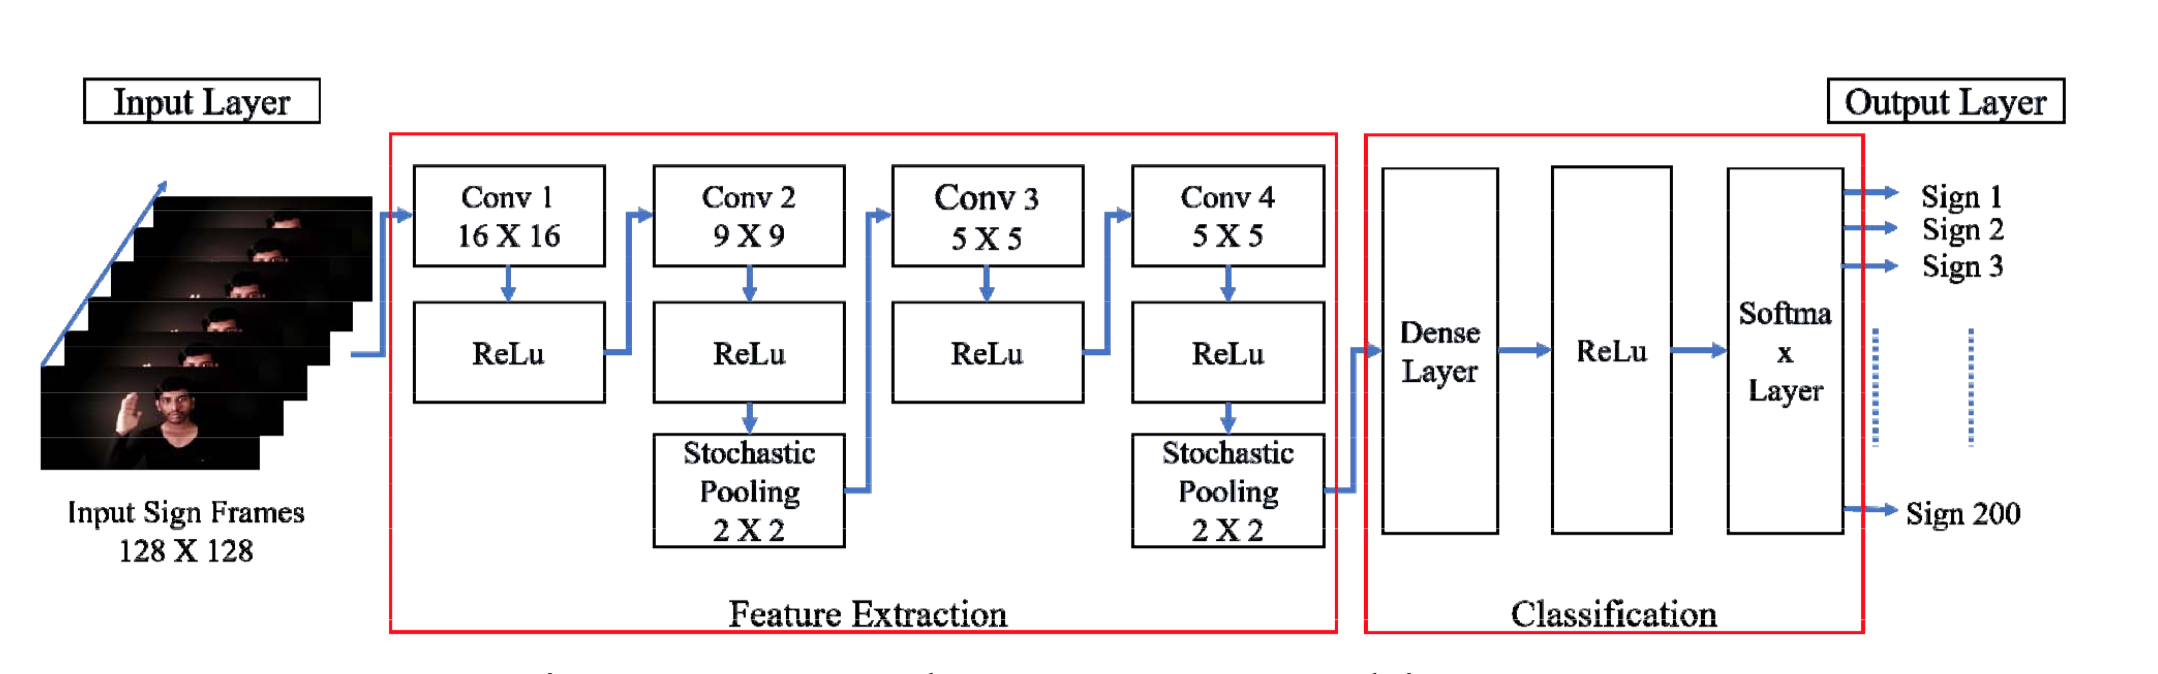
\includegraphics[width=\textwidth]{./images/selfie.png}
    \caption{Proposed Deep CNN architecture}
    \label{fig:selfie}
\end{figure}




\cite{Hussain2017}, introduced a CNN based classifier  trained through the process of transfer learning
over a pretrained convolutional neural network which is trained on a large dataset.
We are using VGG16 figure \ref{fig:vgg16} as the pretrained model.
The According to the paper the accuracy was 93.09\%,while using AlexNet 
figure \ref{fig:alexnet} was 76.96\%. the same problem here with the other papers 
which is the small number of sign that begin trained on 7 signs, and the accuracy
need to be improved as well.
\bigbreak

\begin{figure}[h]
    \centering
    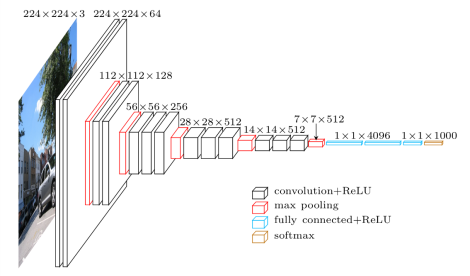
\includegraphics[width=.9\textwidth]{images/vgg16.png}
    \caption{VGG16 architecture. Retrieved from www.cs.toronto.edu}
    \label{fig:vgg16}
\end{figure}
\begin{figure}[h]
    \centering
    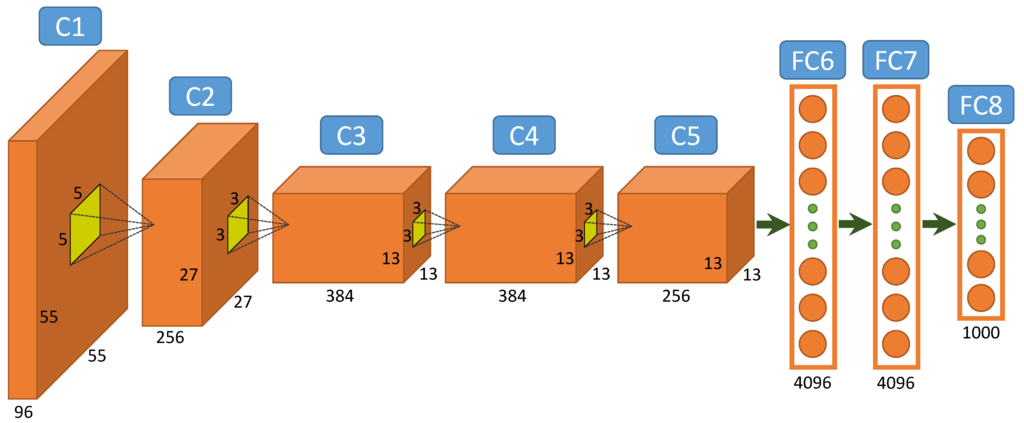
\includegraphics[width=.8\textwidth]{images/alexnet.png}
    \caption{AlexNet architecture. Retrieved from www.saagie.com}
    \label{fig:alexnet}
\end{figure}


\clearpage

    \cite{Pyo2016}, introduced a depth-based hand data with convolution
    neural networks (CNNs).The hand gesture dataset has roughly 6,000 RGB-D images in
    each of 12 labels. In all, there are approximately 60,000
    training images, 1S,000 validation images, and 12,000 training images.
    each time they were increasing the number of layers and testing the accuracy \ref{fig:depth_cnn}.
    They came with result that more number of layers, does not guarantee the increase of accuracy.
\bigbreak

\begin{figure}[h]
    \centering
    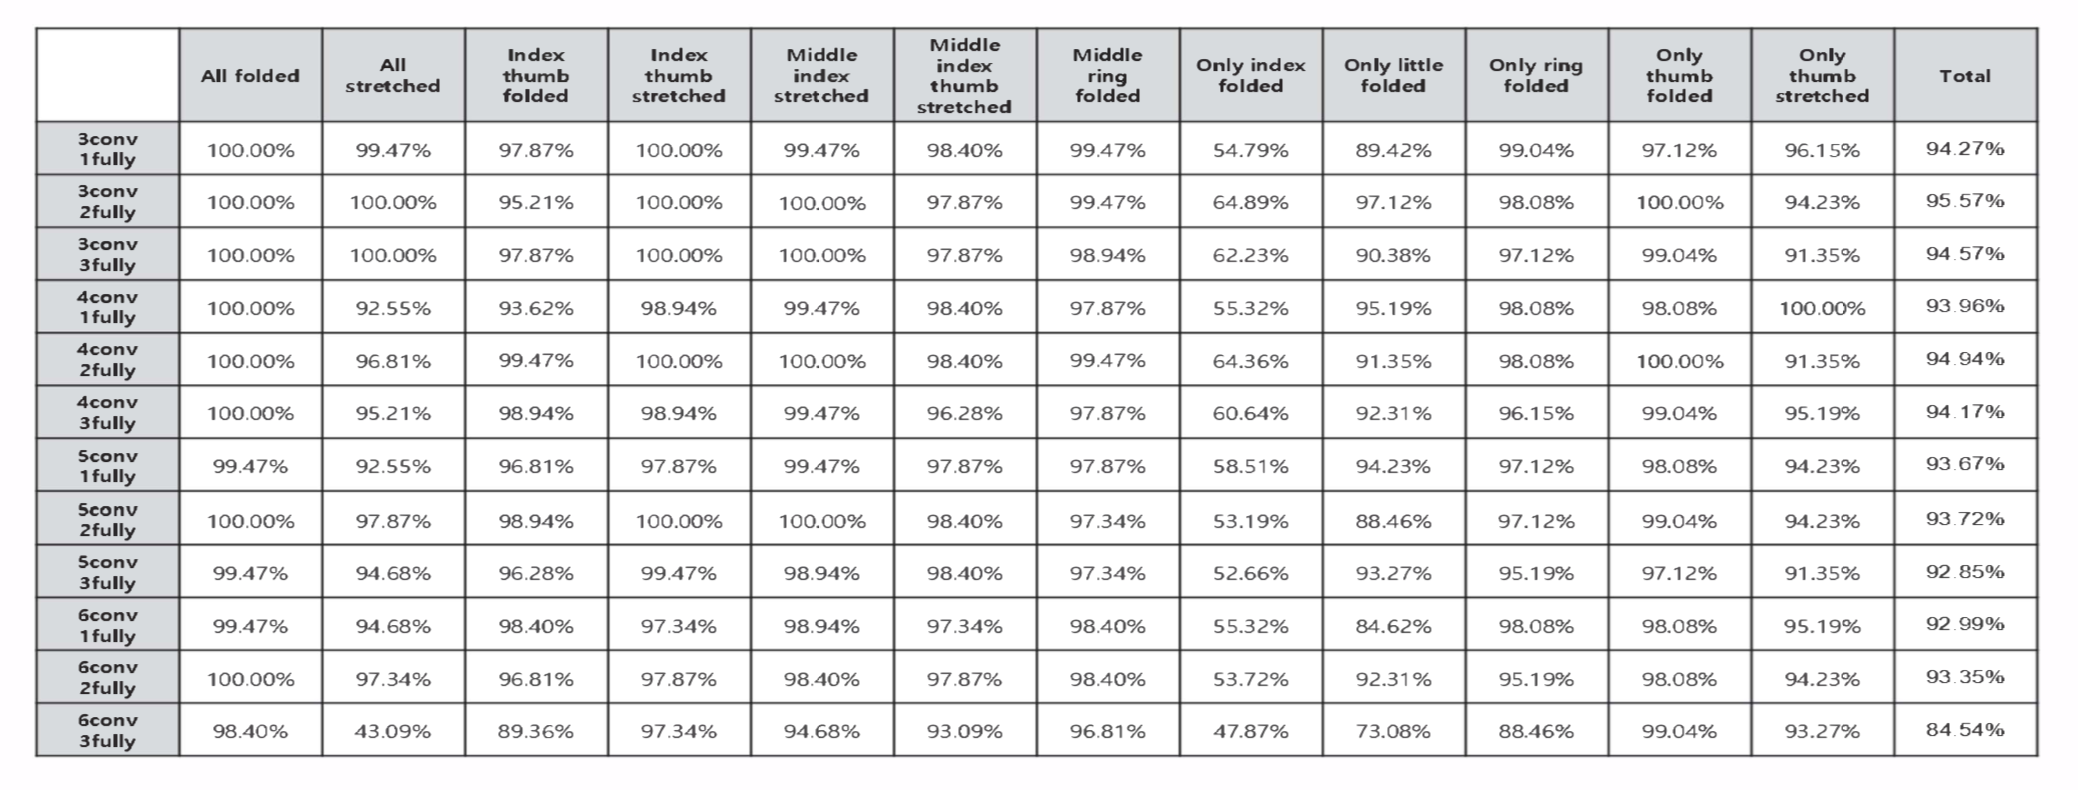
\includegraphics[width=\textwidth]{images/depth_cnn.png}
    \caption{Classification results of  modifiednetworks}
    \label{fig:depth_cnn}
\end{figure}

\bigbreak
    \cite{Devineau2018}, introduced a 3D hand gesture recognition approach based on a deep learning model 
    using Convolutional Neural Network (CNN). The proposed model only uses hand-skeletal 
    data and no depth image.
    The model produced by  multi-channel convolutional neural network
    with two feature extraction modules and a residual
    branch per channel \ref{fig:m_cnn}.
    The achieved accuracy was a 91.28\text{\%} classification accuracy for the 14 gesture
    classes case and an 84.35\text{\%} classification accuracy for the 28
    gesture classes case.
    \begin{figure}[h]
    \centering
    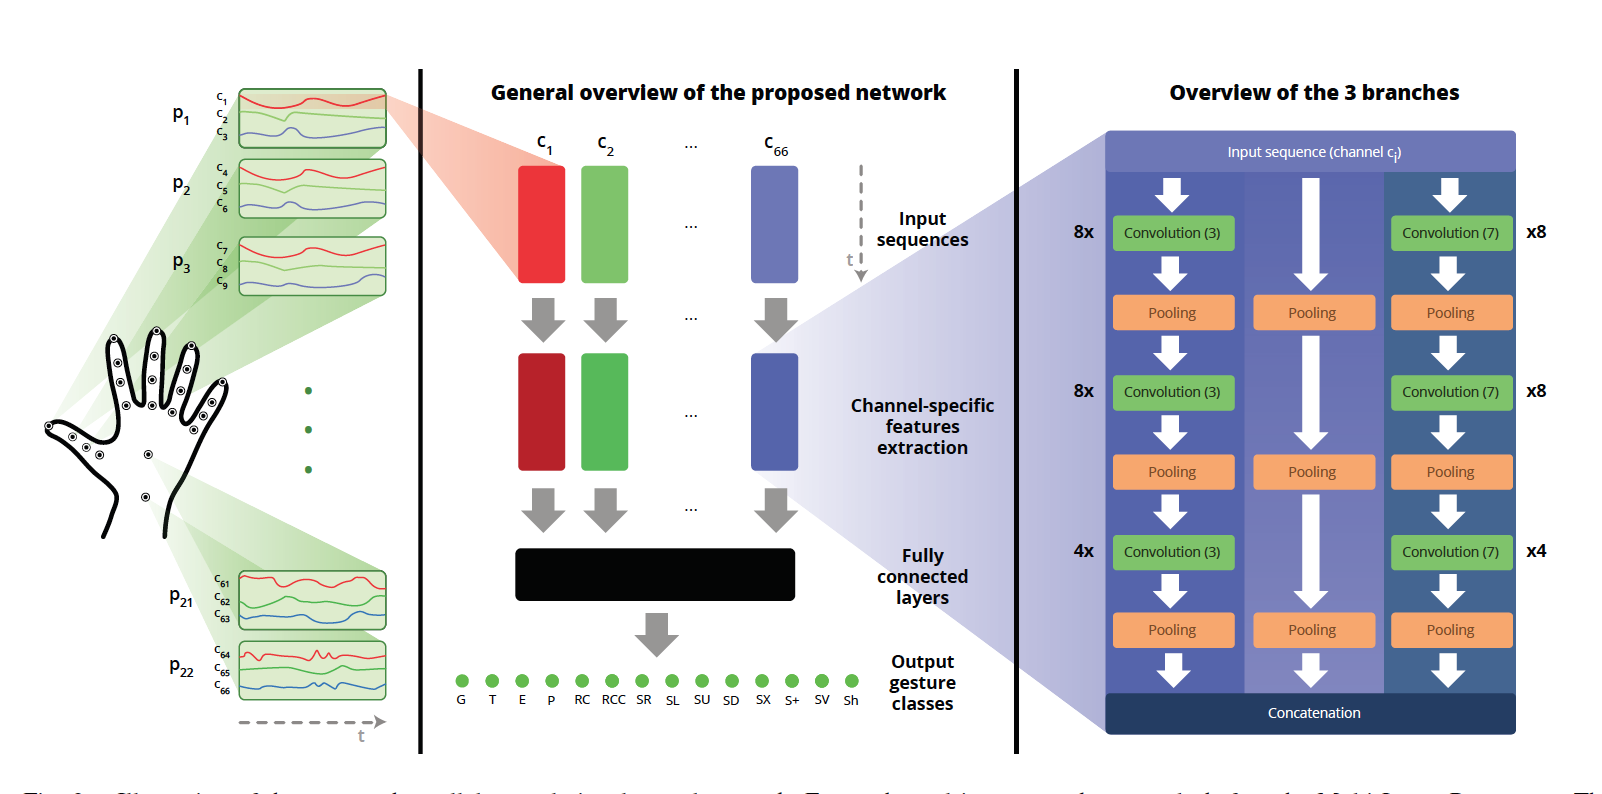
\includegraphics[width=\textwidth]{images/m_cnn.png}
    \caption{parallel convolutional neural network}
    \label{fig:m_cnn}
    \end{figure}


\clearpage
\section{Summary}

This chapter illustrated some works have been done previously on
hand gesture and sign language recognition using Machine Vision and
deep learning (Convolutional Neural Network).
Table \ref{table:summary} shows the summary of the literature review.

\begin{center}
    \begin{table}[h]
        \caption{Summary of the literature review}
        \begin{tabular}{ |p{7cm}|p{2cm}|p{2cm}|p{3cm}| }
            \hline
            Title & Year & Accuracy & Software\\
            \hline
            Tiny Hand Gesture Recognition without Localization via a Deep Convolutional Network & 2017 & 97.1\%& CNN \\
            \hline
            Deep Convolutional Neural Networks for Sign Language Recognition & 2018 & 92.88\% & CNN \\
            \hline
            Hand Gesture Recognition Using Deep Learning & 2017 & 93.09\% & CNN VGG16 \\
            \hline
            Depth-based Hand Gesture Recognition using Convolutional Neural Networks & 2016 & 95.57\% & CNN \\
            \hline
            Deep Learning for Hand Gesture Recognition on Skeletal Data & 2018 & 91.28\% & MC-DCNN \\
            \hline
        \end{tabular}
        \label{table:summary}
    \end{table}
\end{center}
\newpage

\chapter{Methodology}

Image recognition, voice producing, system design block diagram figure \ref{fig:system_diagram} 
and the flowchart of the research is presented in details alongside with the tools
and algorithms in this chapter.


\begin{figure}[h]
    \centering
    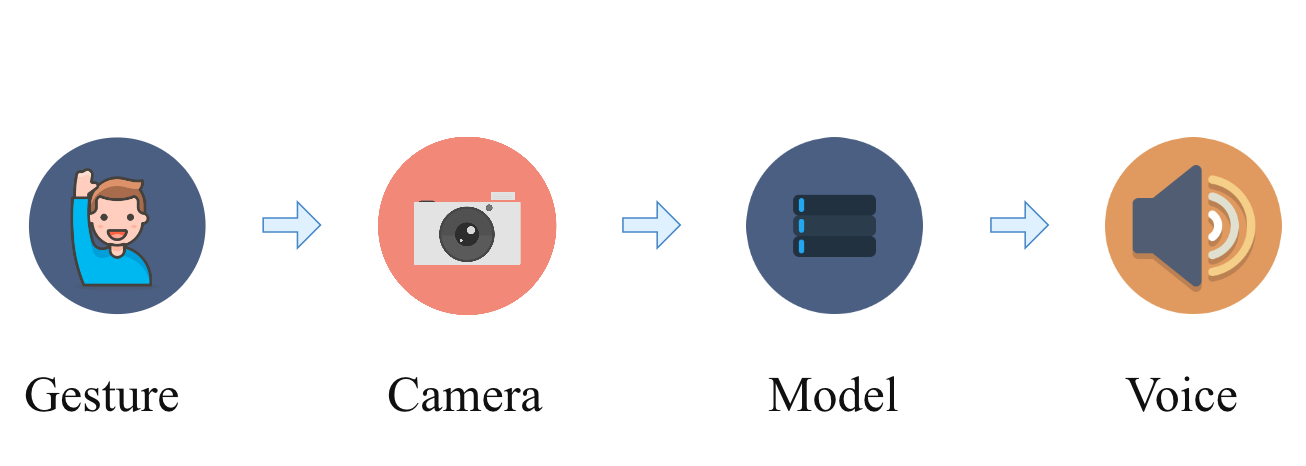
\includegraphics[width=\textwidth]{./images/system_diagram.png}
    \caption{System block diagram}
    \label{fig:system_diagram}
\end{figure}


\clearpage
\section{Deep Learning}
    Deep learning is a machine learning subfield that deals with algorithms based 
    on the structure and function of the brain called artificial neural networks. 
    In other words, it mirrors the brain's functioning.Deep learning algorithms are similar to the structure of 
    the nervous system in which each neuron connects and passes information.
    Deep learning models work in the layers and three layers of a typical model at least \ref{fig:deep_learining}. 
    Each layer accepts and passes the information from the previous layer to the next layer.

    \begin{figure} [h]
        \centering
        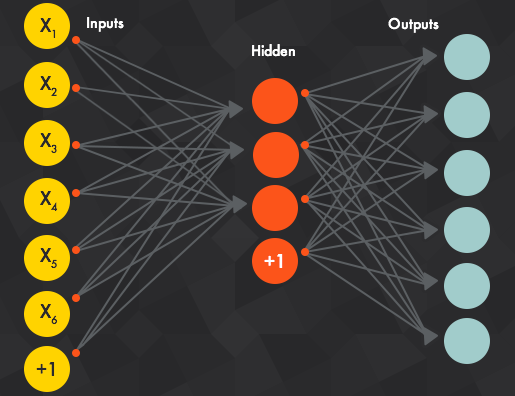
\includegraphics[width=\textwidth]{./images/deep_learning.png}
        \caption{Typical deep learning model. Retrieved from www.medium.com}
        \label{fig:deep_learining}
    \end{figure}

    Deep learning models tend to perform well with quantity of data while old machine 
    learning models do not improve after a saturation.

    One of differences between machine learning and deep learning model is on the feature extraction area. 
    Feature extraction is done by human in machine learning whereas deep learning model figure out by itself.

    \subsection{Activation Function}
    Activation functions are functions that decide what the output of the node should be given the inputs into the node? 
    Since the activation function determines the actual output, the outputs of a layer are often referred to as "activations."
    The most well known activation functions are Sigmoid \ref{fig:sigmoid}, Tanh \ref{fig:tanh} and
    Rectified Linear Unit ReLU \ref{fig:relu}.

    \subsubsection{Sigmoid Function:}
    Non linear activation function with output in range (0,1).
    $$ A = \frac{1}{1+e^{-x}} $$

    \begin{figure} [h]
        \centering
        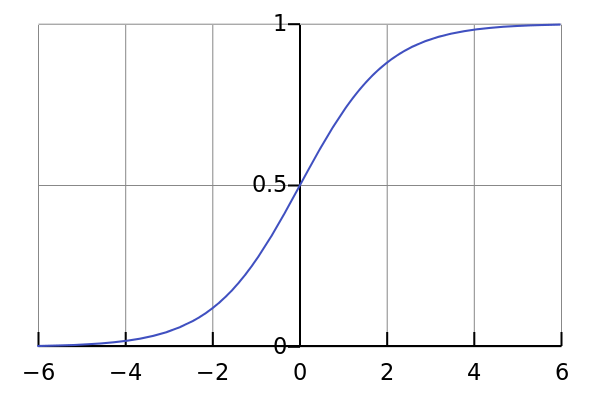
\includegraphics[width=.6\textwidth]{./images/sigmoid.png}
        \caption{Sigmoid Function}
        \label{fig:sigmoid}
    \end{figure}

    \subsubsection{Tanh Function:}
     it is a scaled sigmoid function, bound to range (-1, 1).
    $$ tanh(x) = \frac{2}{1+ e^{-2x}} - 1 $$

    \begin{figure} [h]
        \centering
        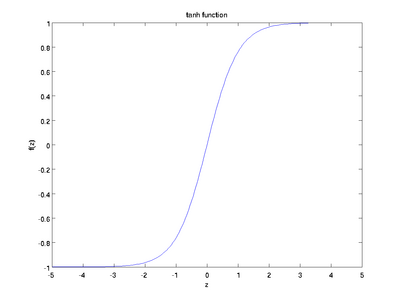
\includegraphics[width=.5\textwidth]{./images/tanh.png}
        \caption{Tanh Function}
        \label{fig:tanh}
    \end{figure}

    \subsubsection{ReLU Function:}
    less computationally expensive than tanh and sigmoid, it is range (-1, infinity).
    $$ A(x) = max(0,x) $$

    \begin{figure} [h]
        \centering
        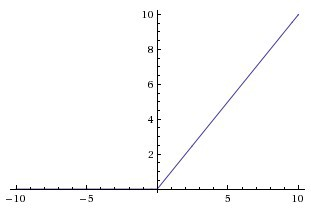
\includegraphics[width=.5\textwidth]{./images/relu.jpeg}
        \caption{ReLU Function}
        \label{fig:relu}
    \end{figure}

\subsection{Weights}
When input data enters a neuron, it is multiplied by a weight value which is assigned to the input. The neuron above the university example, 
for example, has two inputs, test scores and grades, so it has two related weights that can be individually adjusted.
These weights start as random values and as the neural network learns more about what type of input data, 
the weights are adjusted based on any categorization errors resulting from previous weights it can be associated as m in the original linear equation.
$$ y = mx + b$$


\subsection{Bias}
Same as weights, biases are the learnable parameters of the deep learning model.
The bias represents b in the original linear equation.
$$ y = mx + b $$

\section{Convolutional Neural Networks}
Convolutional Neural Networks are very similar to ordinary Neural Networks, 
they are made up of neurons that have learnable weights and biases.
The architectures of ConvNet make the explicit assumption that 
the inputs are images which will be encoded to certain properties in the architecture. 
This makes the forward function more efficient to implement and reduces the number of 
parameters in the network considerably.

Convolutional Neural networks allow computers to see, 
meaning that Convnets is used to recognize images by 
transforming the original image into a class scoring through layers.
CNN was inspired by the visual cortex.
Every time we see something, a series of layers of neurons gets activated, 
and each layer will detect a set of features such as lines, edges. 
The high level of layers will detect more complex features in order to recognize what we saw.

ConvNet has two parts: feature learning (Conv, Relu,and Pool) and classification(FC and softmax).

\subsection{Feature Learning}
    \subsubsection{CONV layer:}
        The objective of a Conv layer is to extract features of the input image.
        A part of the image is connected to the next Conv layer because if all the 
        input pixels are connected to the Conv layer, it is too expensive to compute. 
        Therefore we will apply dot products in all dimensions between a receptive 
        field and a filter. The result of this operation is a single volume integer (future map).
        Then we slide the filter through a Stride over the next receiving field of the same input 
        image and recalculate the dot products between the new receiving field and the same filter.
        This process is repeated until we pass the entire input image. The output is the input on the next layer.

        Some of the word that used interchangeably:
        \begin{itemize}
            \item Filter (Kernel): a small matrix used to detect features.
            \item Feature Map: the output volume formed by sliding the filter over the image and computing the dot product.
            \item Receptive field: a local region of the input image that has the same size as the Kernel.
            \item Depth: the number of filters.
            \item Stride: has the objective of producing smaller output volumes spatially.
            \item Padding: the process of adding extra pixels over around the image.
        \end{itemize}

    \subsubsection{ReLU layer:}
        Turning negative values into zeros. it has nothing to do with size of image and there are no hyperparameters.
    \subsubsection{Pool Layer:}
        Reduce the dimension of the input, the computational complexity of the model and 
        controls the overfitting. There are different types of pooling such as Average pooling, Max pooling and L2-norm pooling.
        However, the Max pooling is the most use, which takes the most important part (the pixel with the highest vule)\ref{fig:pool}. 
        
            \begin{figure}[h]
                \centering
                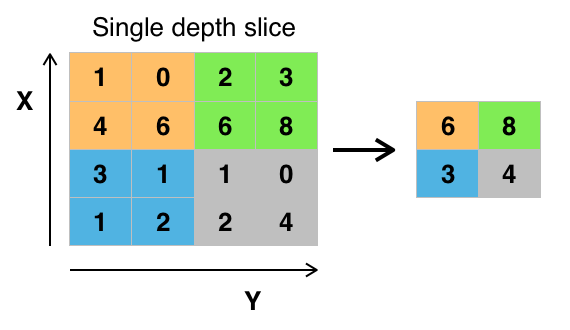
\includegraphics[width=.8\textwidth]{./images/pool.png}
                \caption{Max pooling with 2x2 filter and stride = 2. Retrieved: Wikipedia}
                \label{fig:pool}
            \end{figure}

    \subsection{Classification}
        \subsubsection{Fully Connected Layer(FC):}
            Fully connected layers connect each neuron in a layer to every neuron in another layer.
            The last connected layer uses softmax activation function.
        \subsubsection{Softmax:}
            Activation function generate features input image into many classes based on the dataset.  
        
        \bigbreak
        \bigbreak
        

            \begin{figure} [h]
                \centering
                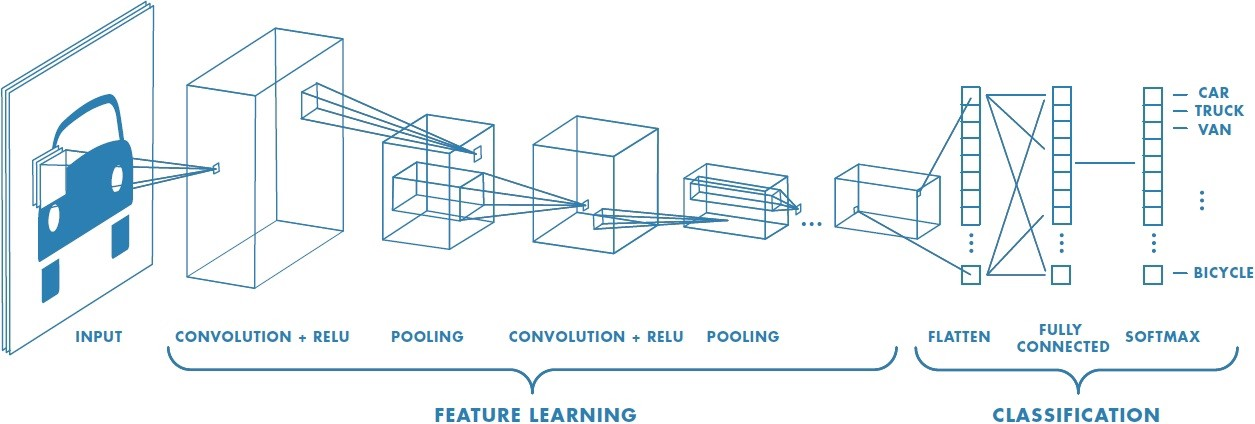
\includegraphics[width=\textwidth]{./images/c_cnn.jpeg}

                \caption{Complete CNN architecture. Retrieved: medium.com}
                \label{fig:c_cnn}
            \end{figure}


\section{Hand detection}

The problem of hand recognition that hand occupied usually less than 25 percent of the image.
To overcome this issue the model should be provided with high accurate detection algorithm,
Right now there are so many good algorithms for object detection which can be utilize to 
detect a human hand We are going to concentrate on the most three famous (Faster R-CNN, SSD and YOLO)

\subsection{Faster R-CNN}

The Faster Region-based Convolutional Network (Faster R-CNN) is a  mixture among  
the Region Proposal Network(RPN)\footnote{algorithm to output bounding boxes to all objects in an image.} 
and the Fast R-CNN\footnote{A main CNN with multiple convolutional layers is taking the entire image as input instead of using a CNN for each region proposals (R-CNN).} model.
\begin{itemize}
    \item A CNN produces feature map form the input images.
    \item A 3x3 sliding window moves through feature map and and maps it into lower dimension.
    \item Every sliding window, produces multiple regions based on fixed ration (anchor boxes).
    \item Each region contain an objectness score and it's bounding box coordinates.
\end{itemize}
\begin{figure}[h]
    \centering
    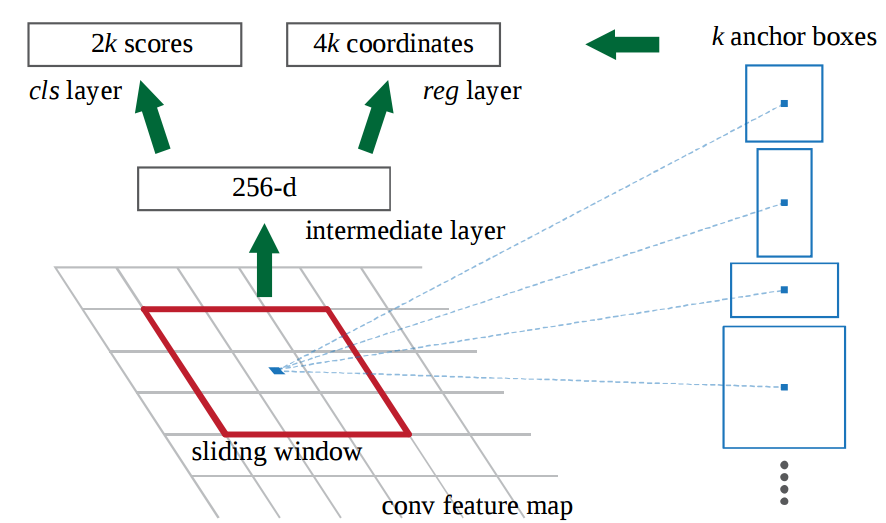
\includegraphics[width=0.6\textwidth]{./images/cfm.png}
    \caption{One sliding window location. Retrieved from https://towardsdatascience.com}
    \label{fig:frcnn}
\end{figure} 
The 2k scores represent the softmax probability of each of the k bounding boxes being on “object.”
If an anchor box has an “objectness” score above a certain threshold, that box’s coordinates (4k coordinates) get passed forward as a region proposal.
Then the region proposals are being fed into a Fast R-CNN, followed by a pooling layer, several fully-connected layers
and softmax classification layer with bounding box regoessor.
Faster R-CNN uses RPN to avoid the 
selective search method \footnote{ Region Proposal algorithm based on grouping of similar region based on color, size, texture and shape compatibility.}, 
it accelerates the training and testing 
processes, and improve the performances. \cite{Ren2017a}
\begin{figure}[h]
    \centering
    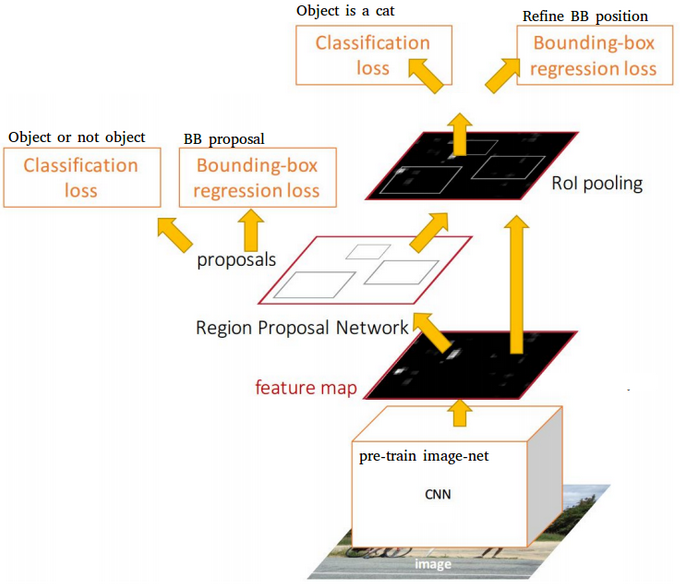
\includegraphics[width=0.7\textwidth]{./images/frcnn.png}
    \caption{Faster R-CNN. Retrieved from https://towardsdatascience.com}
    \label{fig:frcnn}
\end{figure} 

\subsection{Single-Shot Detector (SSD)}

Unlike Faster R-CNN which perform regional proposals 
and region classifications in two steps. SSD does the two in a "single shot"
jointly predict the bounding box and the class while it processes the image.

how it's work?
\begin{itemize}
    \item Generate a set of feature maps with different scales 
    by passing the image through sequence of convolutional layers (10x10, 6x6, 3x3 ...).
    \item Use a 3*3 convolutional filter to evaluate bounding boxes for each location of the feature maps.
    \item predict bounding box of set and the class probability all together.
    \item The best predicted box called as "positive" label, alongside with
    the boxes that have IoU \footnote{Intersection over Union } value $>$ 0.5 
\end{itemize}
Sense SSD skip filtering step, it generates multiple bounding box with multiple shapes
and most of them are negative example.

To fix this issue, SSD does two extra methods.
First, non-maximum suppression:\footnote{Object detection methods often output multiple detections which fully or partly cover the same object in an image.}
to group overlapping boxes into one box by keeping the highest confidence
Then,hard negative mining: to balance classes during the training process; subset the negative examples 
with the highest training loss with a 3:1 ratio of negatives for positives.\cite{Liu2016}

\begin{figure}[h]
    \centering
    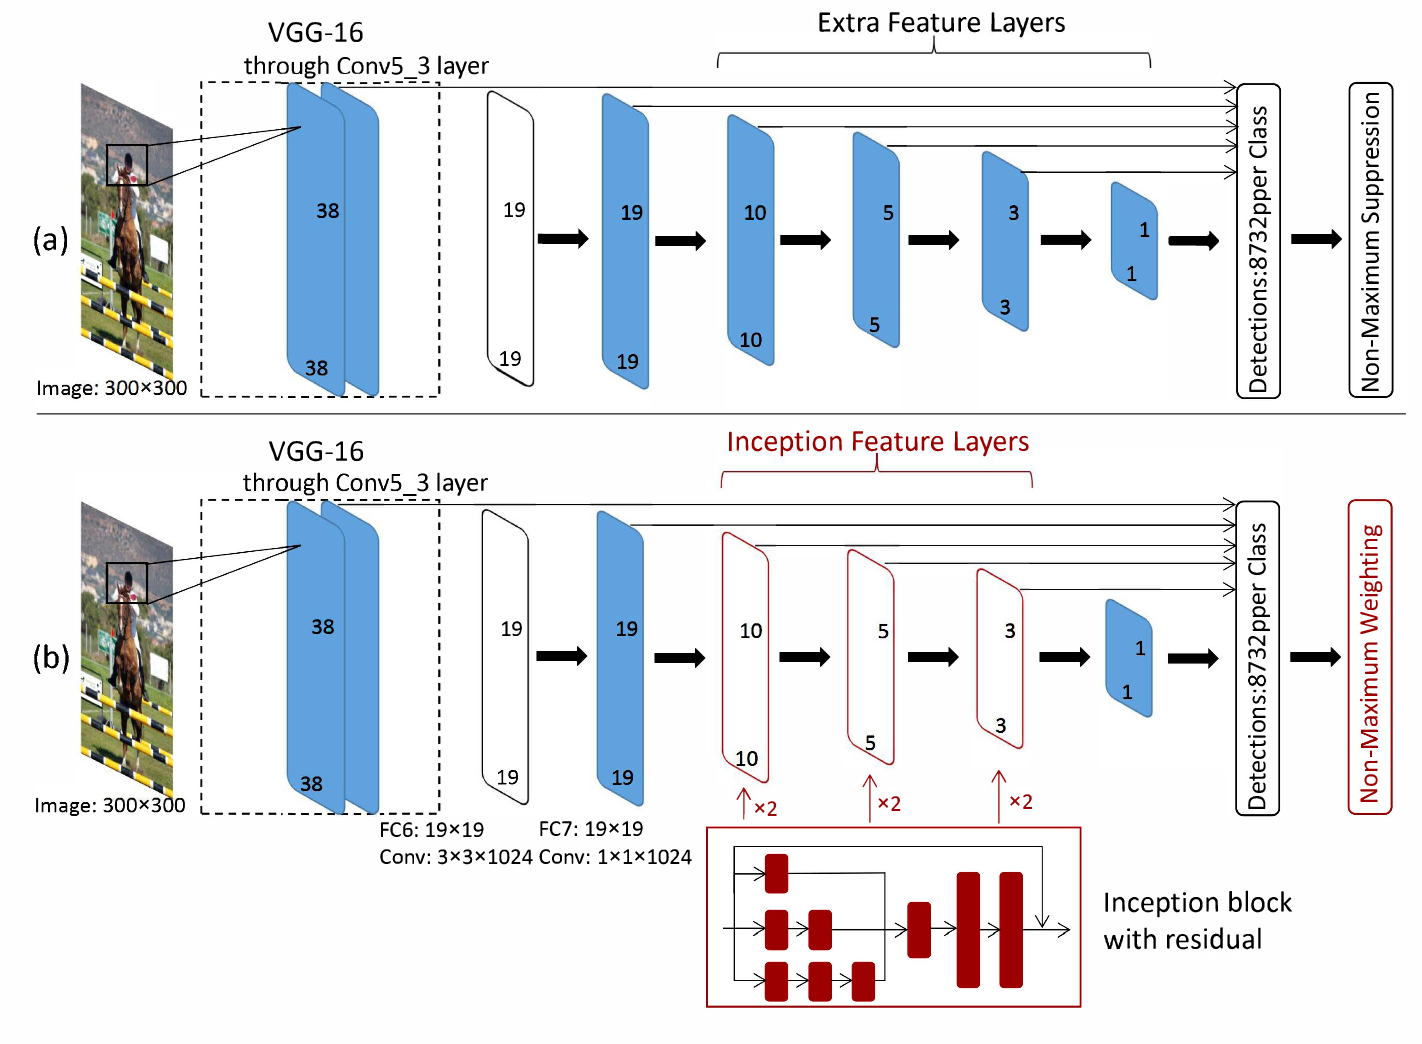
\includegraphics[width=.8\textwidth]{./images/ssd.png}
    \caption{SSD. Retrieved from https://www.semanticscholar.org}
    \label{fig:frcnn}
\end{figure} 



\subsection{You Only Look Once (YOLO)}

Like SSD, YOLO directly predicts bounding boxes and class probabilities
with a single evaluation. The simpleness of YOLO allows real time prediction.
\begin{itemize}
    \item The model divide the input image into SxS grid.
    \item Each cell of the grid predict B bounding boxes with a confidence score.
    \item The score confidence is the probability of detected object multiply by the IoU between the prediction and the truth boxes.
\end{itemize}
The CNN has 24 convolutional layers followed by 2 connected layers.
Reduction layers with 1x1 filters followed by 3x3 convolutional layers 
replace the initial inception modules.
\bigbreak
The Fast YOLO model comes with 9  convolutional layers and less number of filters.
The final layer outputs a S*S*(C+B*5) tensor corresponding to the predictions for each cell of the grid.
C is the number of estimated probabilities for each class.

Similar to SSD, YOLO predicts so many bounding boxes without any object,
So it applies non-maximum suppression method at the end of the network,
to merge high overlapping bounding boxes of the same boxes into a single one.
The author noticed that still some false positive detected.\cite{Redmon2016}


\bigbreak
\bigbreak
\bigbreak


\begin{figure}[h]
    \centering
    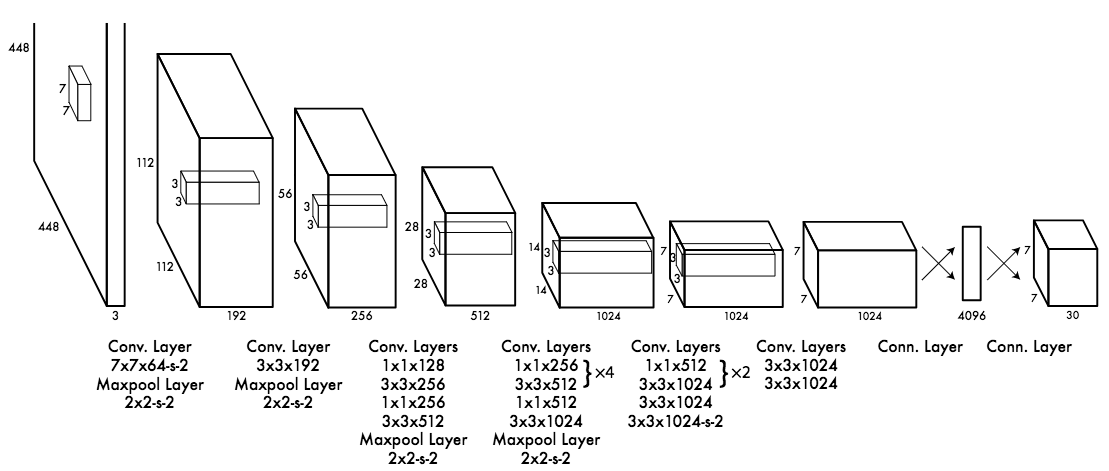
\includegraphics[width=1\textwidth]{./images/yolo.png}
    \caption{YOLO. Retrieved from https://medium.com/}
    \label{fig:frcnn}
\end{figure} 


\newpage

\section{Voice producing}

After processing the image the CNN algorithm classify the gesture
that presented in the image, the corresponding text (word, char, number)
will be generated as voice that Simulate the human voice. 

\section{Tools}

The programming language in use is Python\footnote{Python is an interpreted high-level programming language for general-purpose programming. Created by Guido van Rossum and first released in 1991. https://www.python.org/} along side with many
libraries such as TesorFlow\footnote{TensorFlow is an open-source software library for dataflow programming across a range of tasks. https://www.tensorflow.org/},
Keras\footnote{Keras is a high-level neural networks API, written in Python and capable of running on top of TensorFlow, CNTK, or Theano. https://keras.io/}, 
OpenCV\footnote{OpenCV (Open Source Computer Vision Library) is released under a BSD license and hence it’s free for both academic and commercial use. https://opencv.org/}, 
NumPy\footnote{NumPy is the fundamental package for scientific computing with Python. http://www.numpy.org/}, 
Pandas\footnote{Pandas is an open source, BSD-licensed library providing high-performance, easy-to-use data structures and data analysis tools for the Python programming language. https://pandas.pydata.org/}
and Matplotlib\footnote{Matplotlib is a Python 2D plotting library which produces publication quality figures in a variety of hardcopy formats and interactive environments across platforms. https://matplotlib.org/}.
The model is being trained by using Google Cloud Computing\footnote{Google Compute Engine delivers virtual machines running in Google's innovative data centers and worldwide fiber network. https://cloud.google.com/} service with Ubuntu as operating system.


\renewcommand\bibname{References}            
\bibliography{scope.bib}
\bibliographystyle{apacite}
\end{document}